\documentclass{beamer}
\usepackage[T1]{fontenc}
\usepackage{bookman}
\usetheme[numbering=fraction, progressbar=foot, ,block=fill]{metropolis}  %source : https://fr.overleaf.com/latex/templates/metropolis-beamer-theme/qzyvdhrntfmr et https://mirror.foobar.to/CTAN/macros/latex/contrib/beamer-contrib/themes/metropolis/doc/metropolistheme.pdf

\usepackage{enumitem}
\usepackage{pifont} % puces des listes
\usepackage{blindtext}
\usepackage{hyperref}
\usepackage{fourier}  %symbole \danger
\usepackage[french]{babel}
\usepackage{colortbl} % color tabular
\usepackage{booktabs} %toprule
\usepackage{comment}
\usepackage{color}
\usepackage{multirow}
\usepackage{graphicx} %Loading the package
\graphicspath{{picture/}}


%http://lesfichesabebert.fr/latex/TableauxCouleur.html

%%%%%%%%%%%%%%%%%%%%%%%%%%%%%%%%%%%%%%%%%%%%%%%%%%%%%%%%%
%Information to be included in the title page:

\title{PacMan -- Concepts et maquettes}
\subtitle{SIG3 -- Projet de semestre}
\author{Aline Baeriswyl \& Maxime Fourquaux}
\date{Vendredi 18 novembre 2022}
\logo{
\includegraphics[width=0.75cm]{logoGGT.png}}

\institute[HEIG]%
{
    HEIG-VD  -- EC+G \\
    Orientation GGT
}

%%%%%%%%%%%%%%%%%%%%%%%%%%%%%%%%%%%%%%%%%%%%%%%%%%%%%%%%%
% SOURCES :



%%%%%%%%%%%%%%%%%%%%%%%%%%%%%%%%%%%%%%%%%%%%%%%%%%%%%%%%%

\def\labelenumi{\theenumi}
\setbeamertemplate{enumerate item}{\alph{enumi}}
\setbeamertemplate{enumerate subitem}{\roman{enumii}.}
\usepackage{outline}%
\def\labeloutlni{\theoutlni}%
\def\theoutlni{\alph{outlni}.}%
%\renewcommand{\labelenumi}{\alph{enumi}.)

%\metroset{block=fill} %remplir les blocks
\newcommand{\obligatoire}{{\color{red} \textbf{Obligatoire}}}
\newcommand{\optionnel}{{\color{orange} \textit{Optionnel}}}
\newcommand{\test}{{\color{blue} \textit{Test sur zone restreinte}}}

\definecolor{o}{rgb}{1,0.647,0}

%%%%%%%%%%%%%%%%%%%%%%%%%%%%%%%%%%%%%%%%%%%%%%%%%%%%%%%%%
\begin{document}

% Page de titre
\frame{\titlepage}


% \section{Maquette du projet}
\begin{frame}{Maquette du projet}
    \begin{figure}
        \centering
        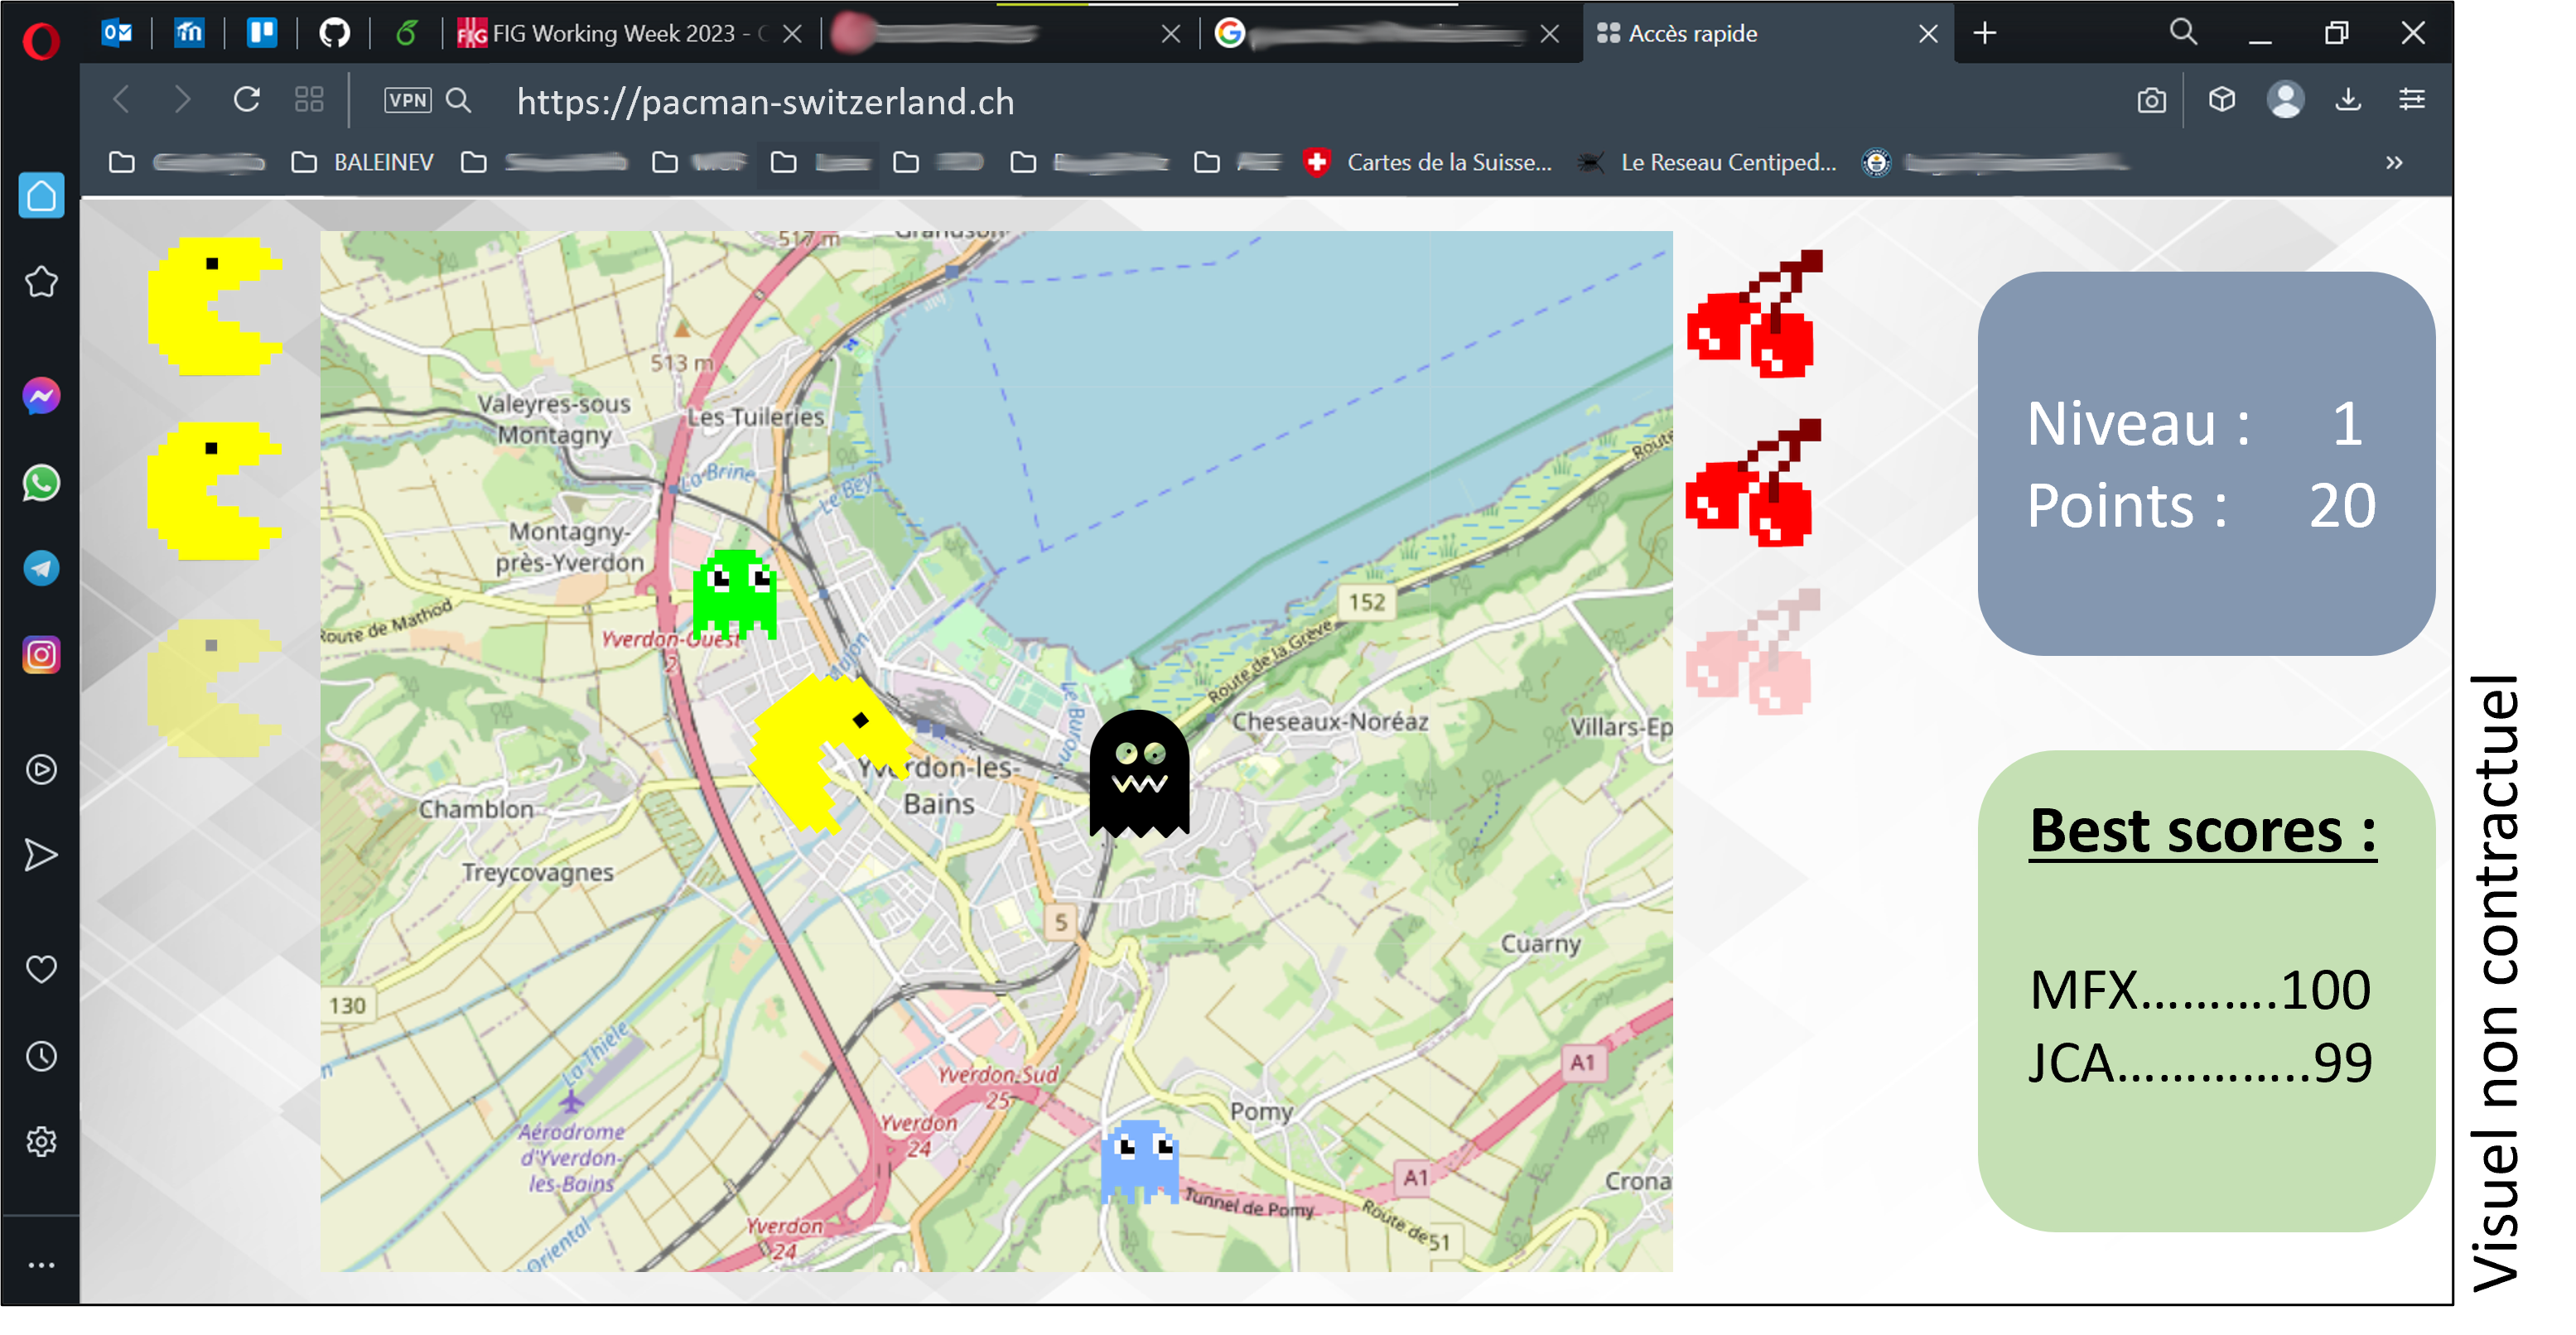
\includegraphics[width=10cm]{maquette.png}
    \end{figure}
\end{frame}

\begin{frame}{Rôles}
    \begin{table}
        \centering
            \begin{tabular}{lp{2cm}p{0.5cm}lp{2cm}}
                \multirow{2}{*}{
\includegraphics[height=1.5cm]{pacMan.png}}      & \textbf{PACMAN}                         & & \multirow{2}{*}{
\includegraphics[height=1.5cm]{ghost.png}}    & \textbf{GHOST}                                              \\
                                                                                 & {\footnotesize Héros du jeu}            & &                                                               & {\footnotesize Méchant du jeu. Sont là pour manger Pac-Man} \\
                \multirow{2}{*}{
\includegraphics[height=1.5cm]{finalBoss.png}}   & \textbf{Final boss}                     & & \multirow{2}{*}{
\includegraphics[height=1.5cm]{cherry.png}}   & \textbf{Cherry}                                             \\
                                                                                 & {\footnotesize Boss final du jeu}       & &                                                               & {\footnotesize Vie/essai dans le jeu}                       \\
                \multirow{2}{*}{
\includegraphics[height=1.0cm]{littlePoint.png}} & \textbf{Point}                          & & \multirow{2}{*}{
\includegraphics[height=1.5cm]{bigPoint.png}} & \textbf{Bonus}                                              \\
                                                                                 & {\footnotesize Pour compter les scores} & &                                                               & {\footnotesize Avantage pour manger les ghosts}             \\
            \end{tabular}
    \end{table}
\end{frame}

\begin{frame}{Aspect technique}
    \begin{itemize}[label=$\rhd$]
        \item Webmapping avec :
        \begin{itemize}[label=>]
            \item Fond de plan (OSM, swisstopo)
            \item Route (roadmap d'OSM)
        \end{itemize}
        \item Base de données pour enregistrer les scores
    \end{itemize}
\end{frame}

\begin{frame}{Règles du jeu}
    \begin{itemize}[label=$\rhd$]
        \item Ne pas se faire manger par les ghosts
        \item Gagner le plus de points possibles en :
        \begin{itemize}[label=>]
            \item grignotant les points
            \item avoir des bonus pour manger les ghosts
        \end{itemize}
    \end{itemize}
\end{frame}

\begin{frame}{Tâches à réaliser}
    \begin{itemize}[label=$\rhd$]
        \item Création de la page d'accueil \\
              {\scriptsize Minimum : pouvoir tester et travailler \\
              Amélioration en continue durant le projet}
        \item Créer les déplacements de PACMAN sur les routes \\
              \test
        \item Créer les intersections de PACMAN par l'utilisateur \\
              \test
        \item Créer les mouvements des fantômes \\
              \test
        \item Généralisation des points précédants à l'ensemble de la ville \\
        \item Créer la gestion des scores (enregistrement des scores, affichages, ...) \\
              \optionnel
    \end{itemize}
\end{frame}

\begin{frame}{Références et sources}
    \begin{itemize}[label=$\rhd$]
        \item \href{https://fr.wikipedia.org/wiki/Pac-Man}{PACMAN, Wikipédia}
        \item \href{https://dev.to/code2bits/pac-man-patterns--ghost-movement-strategy-pattern-1k1a}{PACMAN Patterns - Ghosts movement}
        \item \href{https://gameinternals.com/understanding-pac-man-ghost-behavior}{Understanding Pac-Man Ghost Behavior}
        \item \href{https://www.lefigaro.fr/secteur/high-tech/2015/03/31/32001-20150331ARTFIG00349-google-fait-debouler-pac-man-dans-google-maps.php}{Google fait débouler Pac-Man dans Google Maps}
    \end{itemize}
\end{frame}


\begin{frame}{Planification prévisionnelle}
    \scriptsize
    \begin{table}
        \centering
        \begin{tabular}{l|l|l|l|l|l|l|l|l|l|}
            \textbf{Tâches}                  & \rotatebox{90}{\textbf{18.11.22}} & \rotatebox{90}{\textbf{25.11.22}} & \rotatebox{90}{\textbf{02.12.22}} & \rotatebox{90}{\textbf{09.12.22}} & \rotatebox{90}{\textbf{16.12.22}} & \rotatebox{90}{\textbf{23.12.22}} & \rotatebox{90}{\textbf{13.01.23}} & \rotatebox{90}{\textbf{20.01.23}} & \rotatebox{90}{\textbf{27.01.23}} \\ \hline
            Création page internet           & \cellcolor{o}                     &                                   &                                   &                                   &                                   &                                   &                                   &                                   &                                   \\ \hline
            Sources et import des shp        &                                   &  \cellcolor{o}                    &                                   &                                   &                                   &                                   &                                   &                                   &                                   \\ \hline
            Déplacement PacMan sur une route &                                   &                                   & \cellcolor{o}                     & \cellcolor{o}                     &                                   &                                   &                                   &                                   &                                   \\ \hline
            Interaction PacMan intersection  &                                   &                                   &                                   &                                   & \cellcolor{o}                     & \cellcolor{o}                     &                                   &                                   &                                   \\ \hline
            Déplacement ghosts               &                                   &                                   &                                   &                                   &                                   &                                   & \cellcolor{o}                     &                                   &                                   \\ \hline
            Design page internet             &                                   & \cellcolor{o}                     & \cellcolor{o}                     & \cellcolor{o}                     & \cellcolor{o}                     & \cellcolor{o}                     & \cellcolor{o}                     &                                   &                                   \\ \hline
            Présentation et rapport          &                                   &                                   &                                   &                                   &                                   &                                   &                                   & \cellcolor{o}                     & \cellcolor{o}                     \\ \hline \hline
            \textbf{Cours}                   &                                   &                                   &                                   &                                   &                                   &                                   &                                   &                                   &                                   \\ \hline
            TE1                              &                                   &                                   &                                   & \cellcolor{o}                     &                                   &                                   &                                   &                                   &                                   \\ \hline
            swisstopo                        &                                   &                                   &                                   &                                   &                                   &                                   &                                   & \cellcolor{o}                     &                                   \\ \hline
            \hline
        \end{tabular}
    \end{table}
\end{frame}
\end{document}